\chapter{Sound}




\section{Overview}
In PixelLight there's no difference between sound and music. Therefore we use only the term sound. The sound component is using backends like the renderer component to enable you to use whatever sound API you want to use. But unlike the renderer component no other PixelLight component depends on the sound component. It's possible to playback 2D and 3D sounds and different sounds and music can be mixed/blended together. Here's a digram the sound component look's like:\\
\begin{figure}
  \begin{center}
    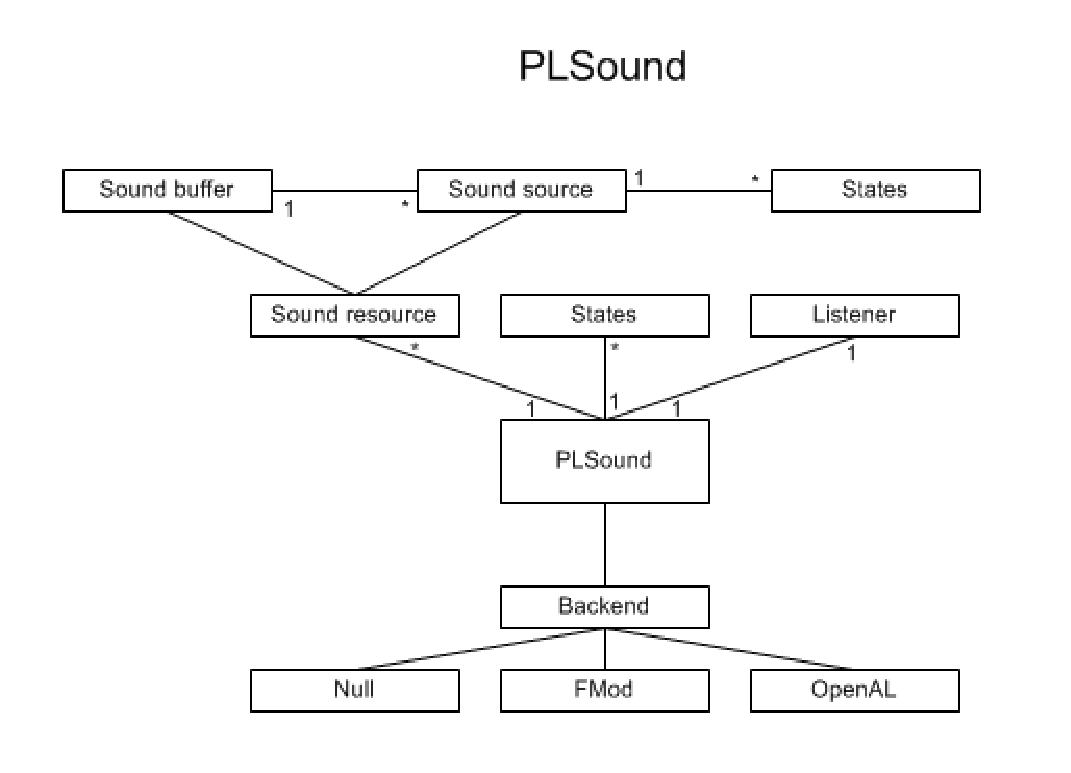
\includegraphics{pics/PLSoundClassDiagram.eps}
  \end{center}
  \caption{Sound component}
  \label{fig:Sound component high-level UML class diagram}
\end{figure}




\section{Sound scene node}
The sound component comes with a scene node called \emph{PLSound::SNSound} you can place into your scene for sound playback. There's also a scene node modifier called \emph{PLSound::SNMSound} if you just want to add sound to a scene node without adding a new one. The sound position is set by this scene node and will do all the dirty work for you, quite easy to deal with dynamic 3D sounds, eh?

This scene plugins can only be used correctly if they are placed inside a \emph{PLSound::SCSound} scene container - but it's not required that they are direct children and can be placed within any sub-container that's inside a sound scene container.

Have a look at the \emph{PLDemoSoundBasic} demo that comes with the PixelLight SDK.
